\chapter{概念设计}
\thispagestyle{empty}
\section{实体}
根据先前的需求分析,本系统所使用的数据库中,包含以下实体集:
\begin{itemize}
  \item \textit{bike}:拥有属性(\textit{\underline{bike\_ID},production\_date,coordinate,status,battery\_remaining\_capacity});
  \item \textit{usage}:拥有属性(\textit{\dotuline{time},coordinate,action});
  \item \textit{parking\_area}:拥有属性(\textit{\underline{parking\_area\_ID},name,coordinate,radius});
  \item \textit{scheduling}:拥有属性(\textit{\dotuline{time},coordinate,action});
  \item \textit{to\_be\_reviewed}:拥有属性(\textit{\dotuline{time},status,proof\_material});
\end{itemize}

\paragraph{\textit{bike}}

该实体集的拓展是在现实中公司所拥有的单车。

该实体集有以下属性:
\begin{itemize}
  \item \textit{\underline{bike\_ID}}:我们认为在同一家共享单车公司中,单车的序列号应当是唯一的,所以将其作为该实体集的主码;
  \item \textit{production\_date}:单车的生产日期;
  \item \textit{coordinate}:该属性用于追踪单车的当前坐标;
  \item \textit{status}:该属性用于记录单车状态,对应数据字典中的bike status项。
\end{itemize}

这里的\textit{production\_date,coordinate}实际上都是复合属性,例如\textit{coordinate}由经度和纬度组成,但是在该数据库的实际应用场景中,通常将它们
作为整体来使用,所以在概念设计中将它们视为整体。

这里的\textit{status}为多值属性,这是因为单车的实际状态可以由多个状态的合理组合而构成,例如一辆单车可以同时处于“闲置”和“低电量”状态。
\paragraph{\textit{usage}}

该实体集的拓展是在现实中共享单车用户对于共享单车的使用。

该实体集有以下属性:
\begin{itemize}
  \item \textit{\dotuline{time}}:事件发生时间;
  \item \textit{coordinate}:事件发生坐标;
  \item \textit{action}:该属性用于标记使用操作是开锁还是关锁;
\end{itemize}

我们认为共享单车的使用这一实体的存在依赖于单车实体。因此我将该实体集设计为弱实体集,它的识别集是\textit{bike},识别关系集是\textit{bike\_usage},识别器为该实体集的\textit{time}属性。

\paragraph{\textit{parking\_area}}

该实体集的拓展是在现实中公司所设立的停车地点。

该实体集有以下属性:
\begin{itemize}
  \item \textit{\underline{parking\_area\_ID}}:我们认为在同一家共享单车公司中,停车区域的ID号应当是唯一的,所以将其作为该实体集的主码;
  \item \textit{name}:停车区域名称;
  \item \textit{coordinate}:停车区域中心坐标;
  \item \textit{radius}:停车区域半径;
\end{itemize}

我们允许不同的停车区域有相同名称。
\paragraph{\textit{scheduling}}
该实体集的拓展是在现实中调度员所产生的调度行为。

该实体集有以下属性:
\begin{itemize}
  \item \textit{\dotuline{time}}:调度发生的时间;
  \item \textit{coordinate}:事件发生坐标;
  \item \textit{action}:该属性用于标记该事件是调度开始还是调度结束;
\end{itemize}
我们认为共享单车的调度这一实体的存在依赖于单车实体。因此我将该实体集设计为弱实体集,它的识别集是\textit{bike},识别关系集是\textit{bike\_scheduling},识别器为该实体集的\textit{time}属性。

\paragraph{\textit{to\_be\_reviewed}}

该实体集的拓展是在现实中调度员所提交的待审查更改。

该实体集有以下属性:
\begin{itemize}
  \item \textit{\dotuline{time}}:提交时间;
  \item \textit{status}:涉及单车状态;
  \item \textit{proof\_material}:用于证明单车状态更改合理性的图片;
\end{itemize}

我们认为待审核更改这一实体的存在依赖于单车实体。因此我将该实体集设计为弱实体集,它的识别集是\textit{bike},识别关系集是\textit{bike\_to\_be\_reviewed},识别器为该实体集的\textit{time}属性。

这里的\textit{status}为多值属性,这是因为单车的实际状态可以由多个状态的合理组合而构成,例如一辆单车可以同时处于“闲置”和“低电量”状态。
同时,\textit{proof\_material}也为多值属性,因为我们允许调度员上传多张照片来佐证状态改变的合理性。

\section{实体属性局部E-R图}

根据先前的需求分析,本系统所使用的数据库中,包含以下关系集:
\begin{itemize}
  \item \textit{bike\_usage}:将单车和单车使用记录关联在一起;
  \item \textit{contain}:将单车和单车停车区域关联在一起;
  \item \textit{bike\_scheduling}:将单车和单车调度记录关联在一起;
  \item \textit{bike\_to\_be\_reviewed}:将单车和待审查记录关联在一起;
\end{itemize}

\paragraph{\textit{bike\_usage}}
如图\ref{usage}所示,关系集\textit{bike\_usage}将实体集\textit{bike}与实体集\textit{usage}联系在一起。

该关系集表达的是“使用单车”这一事件中“单车”和“使用行为”之间的关系。这里的\textit{usage}是弱实体集,它的存在依附于实体集\textit{bike}。
因此,实体集\textit{usage}完全参与关系集\textit{bike\_usage}。

由于对于一次使用行为,有且仅有一辆单车与其相关联,而对于一辆单车,可能有多次使用行为与其相关联,所以图中有指向实体集\textit{bike}的箭头。
\begin{figure}[!htbp]
    \centering
    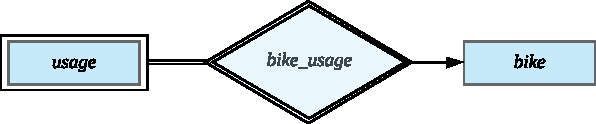
\includegraphics[scale=1]{figures/usage.pdf}
    \caption{\textit{bike\_usage}}\label{usage}
\end{figure}

\paragraph{\textit{contain}}
如图\ref{contain}所示,关系集\textit{contain}将实体集\textit{bike}与实体集\textit{parking\_area}联系在一起。

该关系集表达的是“单车停车区域”和“单车”之间的包含关系。

由于对于一个单车停车区域,可能包含多辆单车,而对于一辆单车,可能被多个停车区域所包含,所以图中并没有指向实体集的箭头。
\begin{figure}[!htbp]
    \centering
    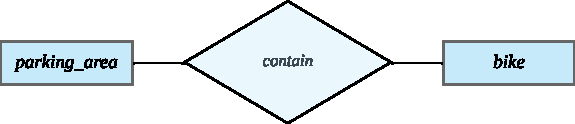
\includegraphics[scale=1]{figures/contain.pdf}
    \caption{\textit{contain}}\label{contain}
\end{figure}

\paragraph{\textit{bike\_scheduling}}

如图\ref{scheduling}所示,关系集\textit{bike\_scheduling}将实体集\textit{bike}与实体集\textit{scheduling}联系在一起。

该关系集表达的是“单车调度”这一事件中“单车”和“调度行为”之间的关系。这里的\textit{scheduling}是弱实体集,它的存在依附于实体集\textit{bike}。
因此,实体集\textit{scheduling}完全参与关系集\textit{bike\_scheduling}。

由于对于一次调度行为,可能涉及多辆单车,而对于一辆单车,也可能涉及多次调度行为,所以图中没有指向实体集的箭头。

\begin{figure}[!htbp]
    \centering
    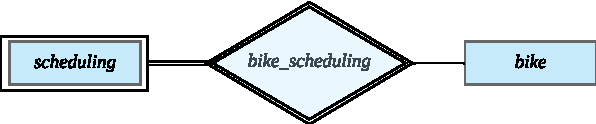
\includegraphics[scale=1]{figures/scheduling.pdf}
    \caption{\textit{bike\_scheduling}}\label{scheduling}
\end{figure}

\paragraph{\textit{to\_be\_reviewed}}
如图\ref{review}所示,关系集\textit{bike\_to\_be\_reviewed}将实体集\textit{bike}与实体集\textit{to\_be\_reviewed}联系在一起。

该关系集表达的是“提交待审查单车状态更新”这一事件中“单车”和“待审查单车状态更新”之间的关系。这里的\textit{to\_be\_reviewed}是弱实体集,它的存在依附于实体集\textit{bike}。
因此,实体集\textit{to\_be\_reviewed}完全参与关系集\textit{bike\_to\_be\_reviewed}。

由于对于一次待审查单车状态更新,有且仅有一辆单车与其相关联,而对于一辆单车,可能有多次待审查单车状态更新与其相关联,所以图中有指向实体集\textit{bike}的箭头。
\begin{figure}[!htbp]
    \centering
    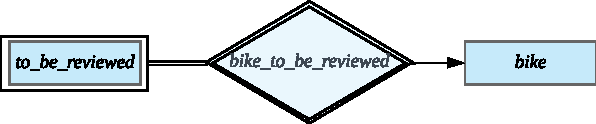
\includegraphics[scale=1]{figures/review.pdf}
    \caption{\textit{to\_be\_reviewed}}\label{review}
\end{figure}

\section{全局E-R图}
图\ref{ER}为全局E-R图。
\begin{figure}[!htbp]
    \centering
    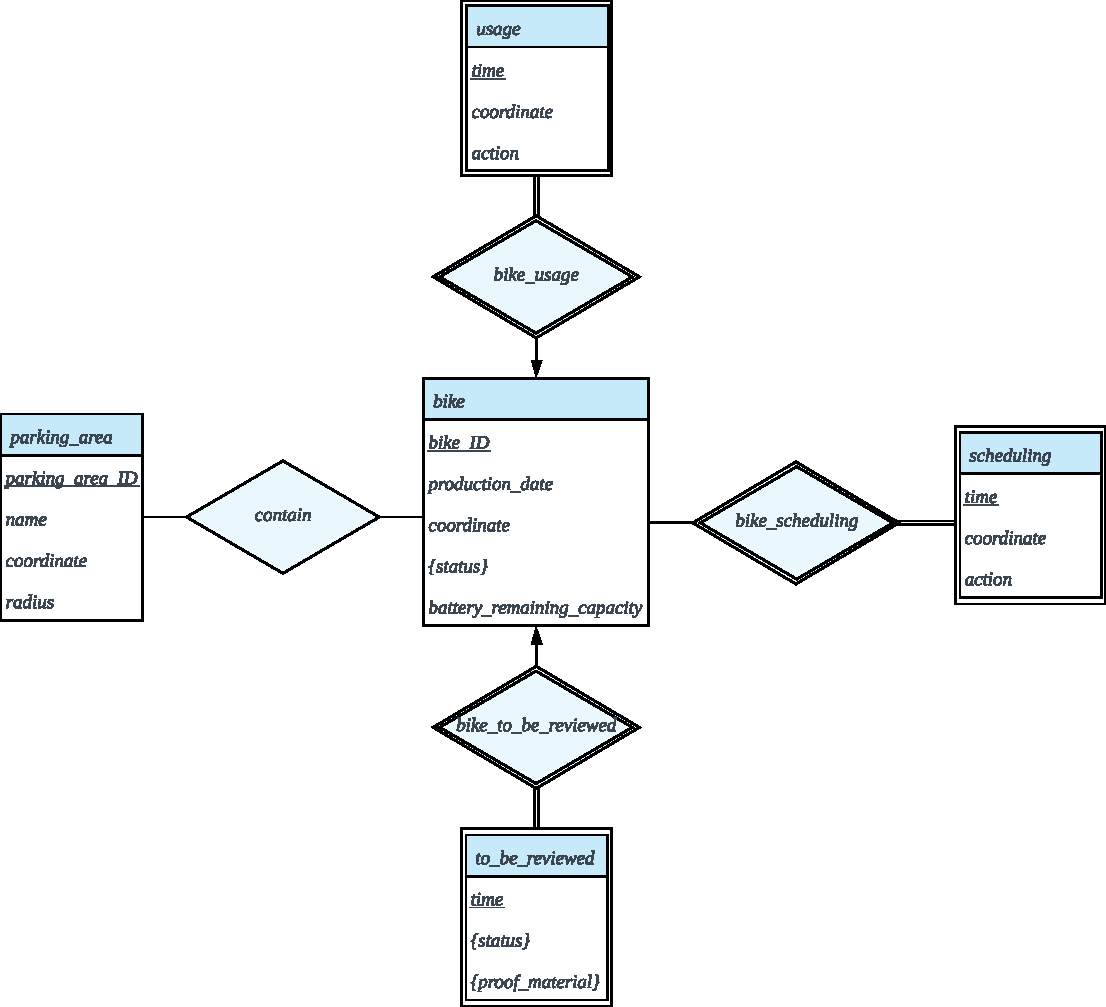
\includegraphics[width=\textwidth]{figures/ER.pdf}
    \caption{全局E-R图}\label{ER}
\end{figure}
